\documentclass[border=6pt]{standalone}
% Shared TikZ styles for the network diagrams.
\usepackage{tikz}
\usetikzlibrary{arrows.meta,positioning}
\definecolor{nodeblue}{HTML}{2A78D6}
\definecolor{endfill}{HTML}{E3EEFB}
\definecolor{shortcut}{HTML}{D64545}
\tikzset{
  v/.style={circle, draw=nodeblue, line width=1pt, minimum size=9mm, inner sep=0pt, font=\small},
  od/.style={v, fill=endfill},
  e/.style={-{Latex[length=2.6mm]}, line width=0.8pt},
  free/.style={e, shortcut},
  c/.style={font=\footnotesize, fill=white, inner sep=1.5pt},
}

\begin{document}
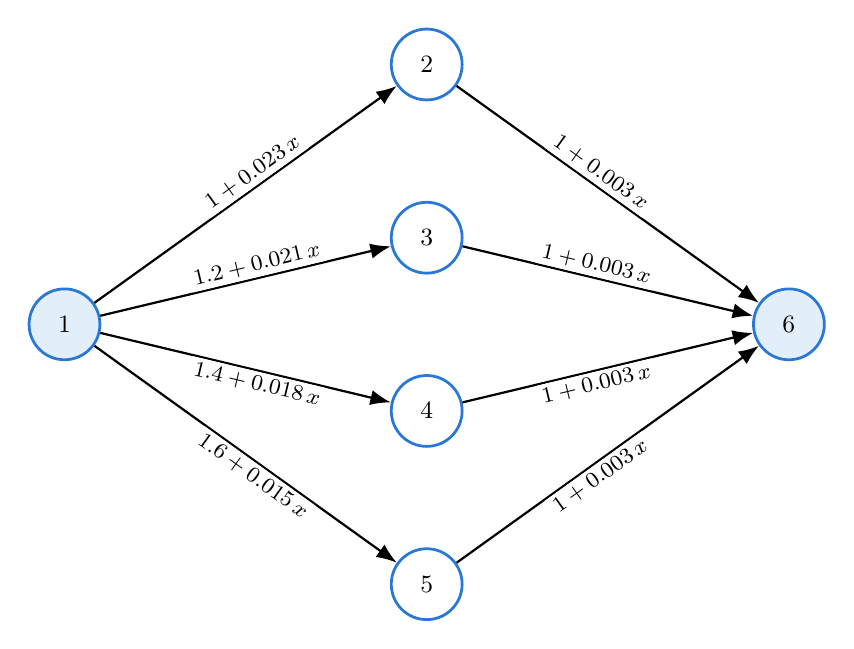
\begin{tikzpicture}
  \node[od] (1) at (0,0) {1};
  \node[v]  (2) at (4.6,3.3)  {2};
  \node[v]  (3) at (4.6,1.1)  {3};
  \node[v]  (4) at (4.6,-1.1) {4};
  \node[v]  (5) at (4.6,-3.3) {5};
  \node[od] (6) at (9.2,0) {6};
  \draw[e] (1) -- node[c, sloped, above, pos=0.55] {$1 + 0.023\,x$} (2);
  \draw[e] (1) -- node[c, sloped, above, pos=0.55] {$1.2 + 0.021\,x$} (3);
  \draw[e] (1) -- node[c, sloped, below, pos=0.55] {$1.4 + 0.018\,x$} (4);
  \draw[e] (1) -- node[c, sloped, below, pos=0.55] {$1.6 + 0.015\,x$} (5);
  \foreach \m/\p in {2/above, 3/above, 4/below, 5/below}
    \draw[e] (\m) -- node[c, sloped, \p, pos=0.45] {$1 + 0.003\,x$} (6);
\end{tikzpicture}
\end{document}
